\subsection{Visualização dos resultados no painel local}
\label{sec:resultados-painel}
As Figuras~\ref{fig:painel-resultados} a~\ref{fig:painel-falhas} são capturas reais de 23 de novembro de 2026, posteriores à campanha. O painel consulta os relatórios públicos verificados; não gera nova amostra, não reclassifica a parcial e não substitui as tabelas. As páginas horizontais favorecem a leitura das telas.

Na Figura~\ref{fig:painel-resultados}, linhas unem cinco pares a 48 eventos/s. HTTP e envio--commit têm eixos independentes; os cartões mostram médias dos p95 por coleta, sem reunir eventos em uma amostra única. A Figura~\ref{fig:painel-cenarios} reúne sete recortes, correspondentes às treze condições por variante: consumidor parado não possui contraparte síncrona, e conclusão com banco parado mantém quatro pares elegíveis.

A Figura~\ref{fig:painel-falhas} separa o resultado original de recuperação, 1/5, da leitura exploratória, 5/5. Os 14 eventos na DLQ continuam fora do PostgreSQL; a visualização não altera o veredito congelado. A demonstração com novas cargas permanece separada, conforme a Seção~\ref{sec:interface}.

\clearpage
\begin{landscape}
\begin{figure}[p]
\centering
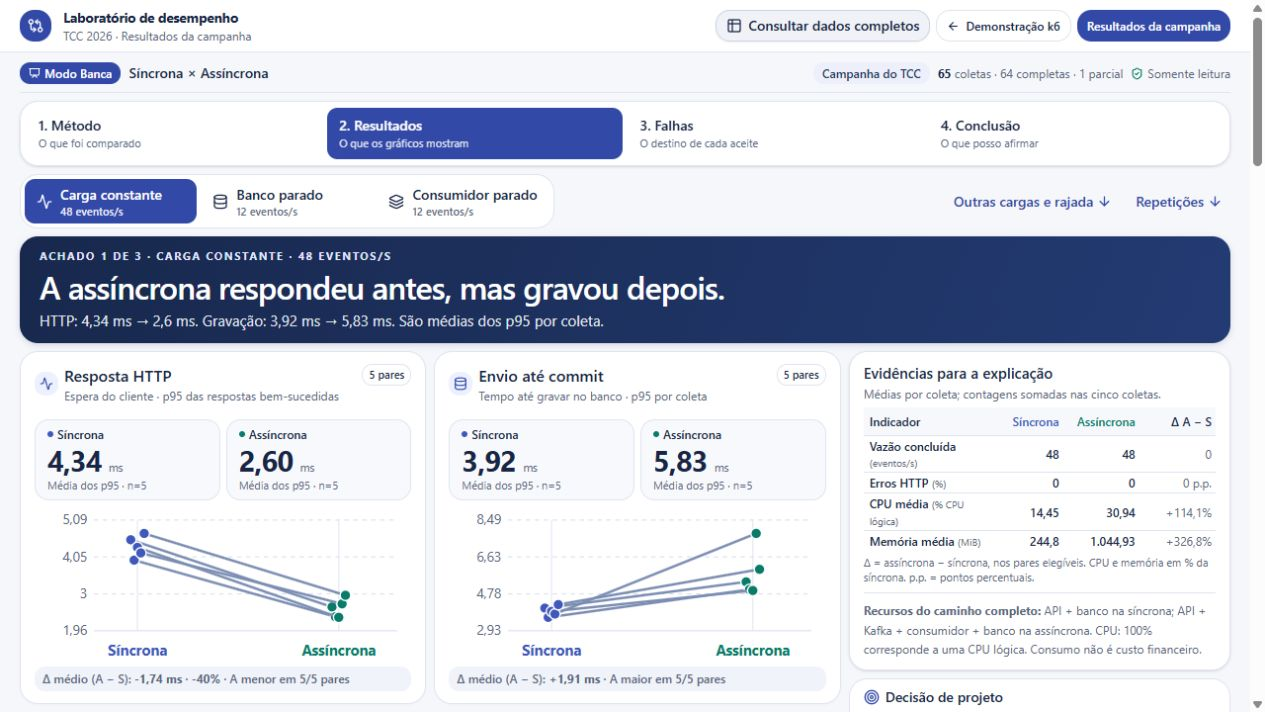
\includegraphics[width=0.98\linewidth,height=0.76\textwidth,keepaspectratio]{Imagens/painel/2026-11-23-resultados-pareados.jpg}
\caption{Painel de resultados: HTTP e envio até commit a 48 eventos/s}
\label{fig:painel-resultados}
\fonte{Captura da interface implementada pelo autor, em 23 nov. 2026, sobre os resultados R2/A1.}
\end{figure}
\clearpage
\end{landscape}

\begin{landscape}
\begin{figure}[p]
\centering
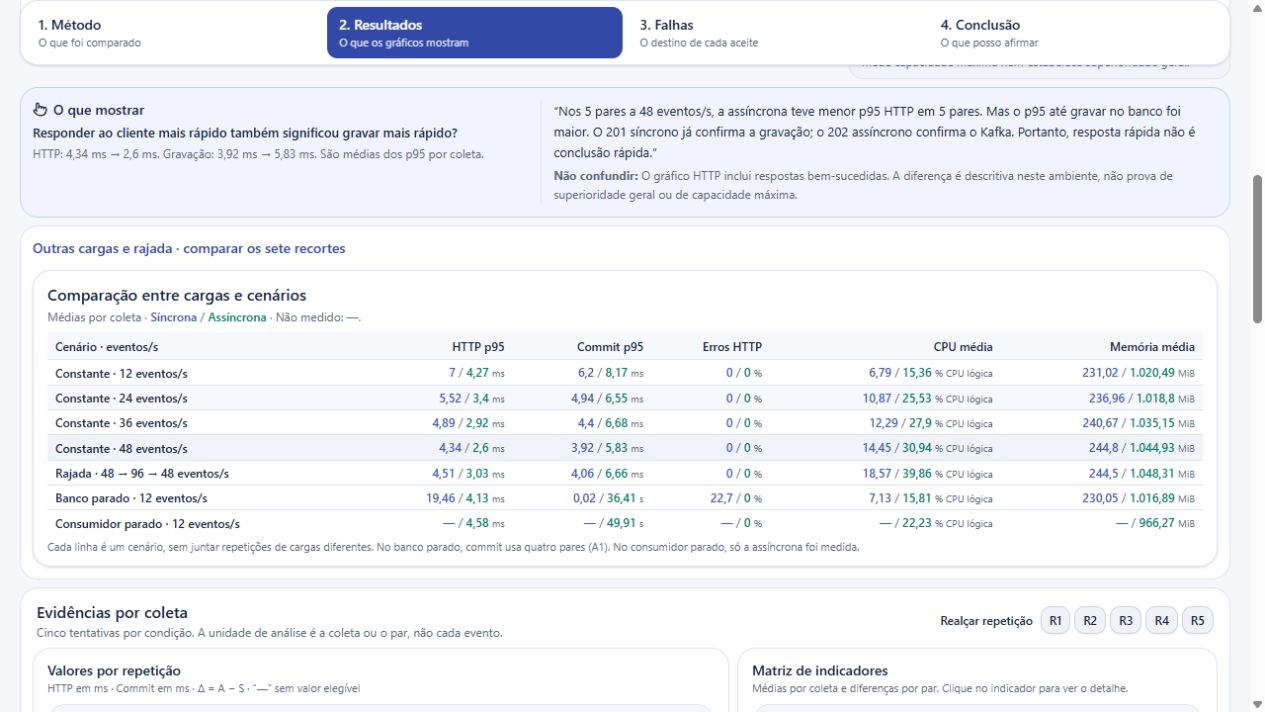
\includegraphics[width=0.98\linewidth,height=0.76\textwidth,keepaspectratio]{Imagens/painel/2026-11-23-cenarios-repeticoes.jpg}
\caption{Consulta dos sete recortes de carga e falha no painel}
\label{fig:painel-cenarios}
\fonte{Captura da interface implementada pelo autor, em 23 nov. 2026, sobre os resultados R2/A1.}
\end{figure}
\clearpage
\end{landscape}

\begin{landscape}
\begin{figure}[p]
\centering
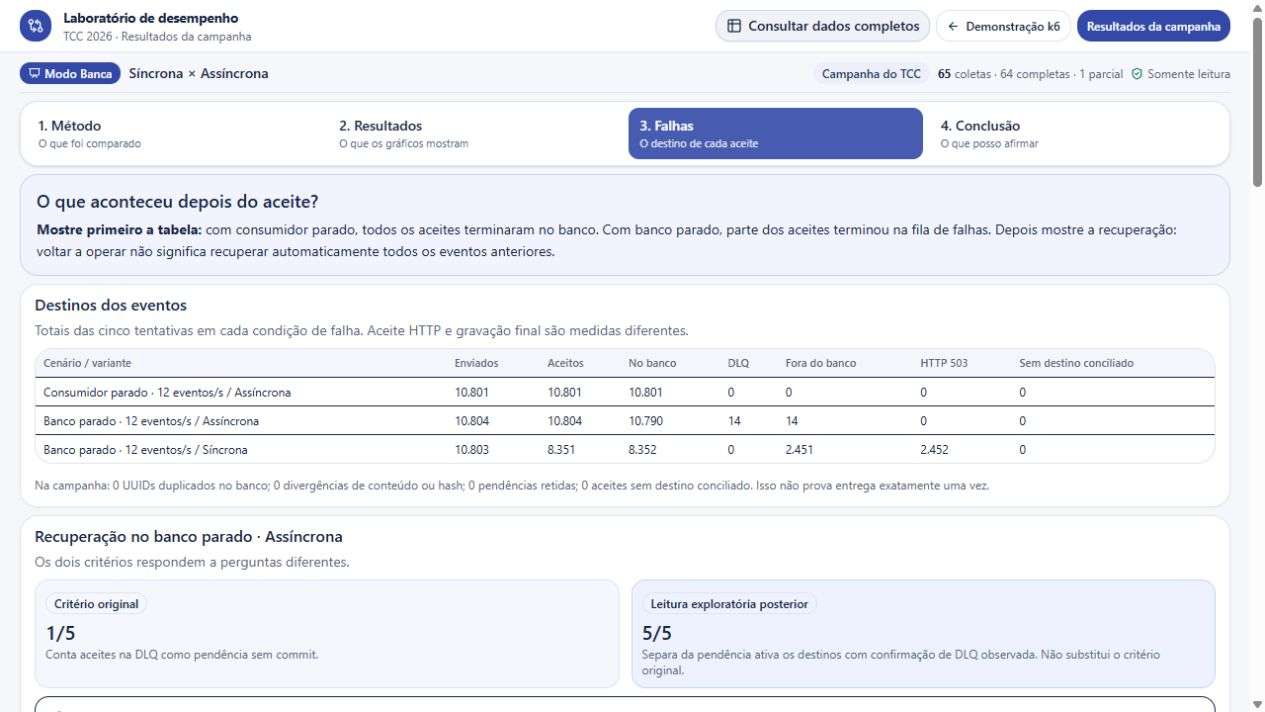
\includegraphics[width=0.98\linewidth,height=0.76\textwidth,keepaspectratio]{Imagens/painel/2026-11-23-falhas-recuperacao.jpg}
\caption{Destinos e recuperação: critério original e leitura exploratória}
\label{fig:painel-falhas}
\fonte{Captura da interface implementada pelo autor, em 23 nov. 2026. A DLQ não representa gravação no banco.}
\end{figure}
\clearpage
\end{landscape}
